
\subsection{Types and Functions}

In the LHC machine, there are various accelerator magnets which can be divided into three main groups based on their function~\cite{cern_main_webpage}: 
\begin{enumerate}
    \item Main dipole magnets. They apply a centripetal Lorentz force to moving particle beams in order to maintain them in the curvature of a 27-km ring. There are 1232 dipoles in the LHC.
    \item Main quadrupole magnets. They constrain the width and the height of a particle beam in order to maintain them inside of a vacuum chamber inside the LHC magnet. There are 392 such magnets inside the LHC.
    \item Corrector magnets. One of their goals is to correct imperfections in the field quality created in the aforementioned magnets. Some of the examples of such magnets are: quadrupoles and skew quadrupoles, sextu-, octu-, deca- or dodecapoles. 
\end{enumerate}

Fig.~\ref{fig:cross_section_lhc_main_dipole} presents the cross-section of the main LHC dipole. The particle beam is travelling inside of a vacuum chamber surrounded by a coil composed of multiple turns of a~superconducting cable. During the operation of the machine, Lorentz forces are exerted on the coil. Therefore, the coils are usually clamped with pre-stressed steel collars holding them together with a sufficient precision. Since the magnets are mounted at room temperature, the pre-stress also serves for maintaining the elements position when the entire structure shrinks during the cooling process. The collars are surrounded by a concentrically mounted iron yoke. The iron yoke increases the central magnetic field that directs a travelling beam.

\begin{figure}[H]
    \centering
    \begin{tikzpicture}
    \node at (0,0) {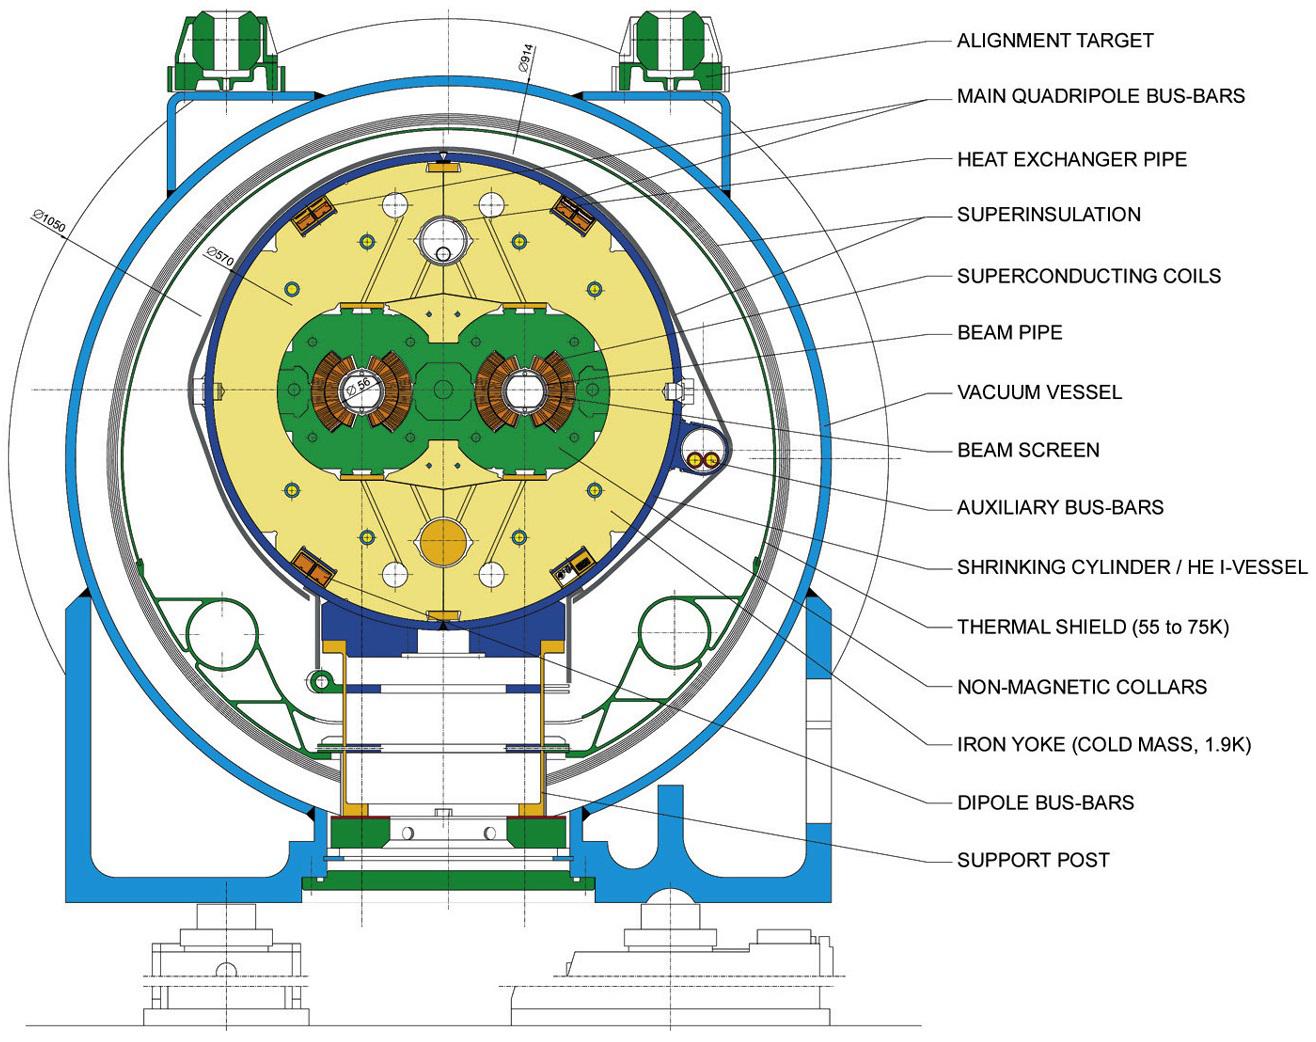
\includegraphics[width=.75\textwidth]{sections/introduction/figures/LHC_main_dipole_cross_section.png}};
    \end{tikzpicture}
    \caption{Cross-section of the LHC main dipole magnet with description of main components~\cite{lhc_main_dipole_cross_section}.}
    \label{fig:cross_section_lhc_main_dipole}
\end{figure}

\subsection{Quench Protection}

When a quench occurs during the operating conditions of a superconducting magnet, it~must to be detected in the shortest possible time. As soon as the quench is detected, the~power converter, that supplies multiple magnets connected in series, is switched off and the magneto-electric energy stored in the circuit is discharged. In principle, the energy should be either deposited in the coil or extracted from the magnet. The quench protection systems can be passive or active. The latter use additional electronics which triggers the quench protections devices. An example of a passive protection system is a diode connected in parallel to a magnet. Since the same voltage is applied to the diode and the magnet, the former allows the current to bypass the latter above a~threshold voltage at which the diode is triggered. Among others, three active protection systems are described: 

\begin{enumerate}
	\item Energy extraction,
	\item Quench heaters,
	\item Couple-Loss-Induced-Quench (CLIQ) system. 
\end{enumerate}

In case of an energy extraction, a part of the energy stored in a magnet is discharged in an external dump resistor connected in series with a superconducting circuit. When the quench is detected, an active switch connects the resistor to the circuit. Thus, a~part of the energy stored in the circuit is discharged in the resistor. This system allows for a faster recovery of a magnet to its operating conditions because it requires less cooling power after the discharge process. The extraction system usually cannot discharge the entire energy because its resistance is limited by the maximum voltage allowed across the magnet terminals. At cryogenic temperatures, the electrical permeability of the insulation between different windings of the coil is reduced. Therefore, the increase of voltage across the coil may lead to a short-circuit inside of a magnet~\cite{salmiquenchheateroptimization}. 

Quench heaters are resistive strips installed along the coils in a close contact with the~windings. The heaters have an external power supply usually based on a charged capacitor. When a quench is detected, the heaters are fired. Due to the firing of the protection system the heater spots, being in a close contact with the windings, quench inside of a coil. This process supports the longitudinal quench propagation initiated at each of the quench heater spot. A~larger resistive volume is created in the magnet and the current discharge occurs more quickly. The quench heaters have an external power supply independent of the superconducting coils. Therefore, they must be electrically insulated from the windings. In fact, the electrical insulation is a thermal barrier causing a~delay between the moment when the heaters are fired and the time when the coil quenches. This delay is a characteristic feature of a quench heater system. The~drawbacks of the quench heaters are as follows~\cite{salmiquenchheateroptimization}: 

\begin{itemize}
    \item On one hand, the quench heater system requires a high thermal diffusivity, i.e. the~insulation between the heater and a coil should be thin to decrease the~delay of a firing system. One the other hand, the system should meet the requirements of an electrical insulation which should be thick enough to prevent short-circuits. These two statements are contradictory with respect to one another. 
	\item There is no possibility to replace quench heating strips of the magnet once they are installed. Therefore, the maintenance of this system is limited in a~long-term of a machine operation. 
\end{itemize}

There also exists a natural effect that enables a magnet to discharge more quickly, called a “quench back”. According to the Faraday’s law, the variation of a magnetic field in time induces eddy currents in an electrical conductor, called AC-losses. If the current drops sufficiently fast, the eddy currents may induce a quench in the parts of a coil which remain superconducting. This phenomenon is called a “quench back”. The CLIQ system is based on the same physical phenomenon. It generates current oscillations in the superconducting windings to create a fast change of a magnetic field. According to~\cite{ravaioli_cliq_phd_thesis}, the CLIQ protection is more efficient with respect to the quench heaters in the operating conditions of a magnet close to the critical surface. CLIQ is implemented as a baseline in some of the magnets for the HL-LHC project.

A superconducting magnet can also be "self-protected" meaning that the energy accumulated in the circuit is discharged by a natural rise of resistivity inside of a magnet. This is the simplest and the cheapest solution. The self-protectability is applicable in magnets characterised by a relatively low current densities and, therefore, low magnetic fields. A low level of the stored energy allows the magnet to limit the temperature rise during the discharge. 
